\documentclass[a4paper,12pt]{article}
\usepackage{a4wide}
\usepackage[T1]{fontenc}
\usepackage{lmodern}
\usepackage[utf8]{inputenc}
\usepackage{xcolor}
\usepackage[czech,english]{babel}
\usepackage[pdftex, final]{graphicx}
% \usepackage[pdftex, final, colorlinks=true]{hyperref}
\usepackage{verbatim}
\usepackage{alltt}
\usepackage{paralist}
\usepackage{mdwlist}
\usepackage{subfig}
\usepackage[final]{pdfpages}
%\usepackage[hyphens]{url}
%\PassOptionsToPackage{hyphens}{url}

\usepackage[final,pdftex,colorlinks=false,breaklinks=true]{hyperref}
\usepackage[hyphenbreaks]{breakurl}

%%%%%%%%%%%%%%%%%%%%%%%%%
% pro podmineny preklad
% false je defaultně


% \newif\ifbc % Pouze do bakalářské práce
%  \bctrue

%%%%%%%%%% fancy %%%%%%%%%%%
\usepackage{fancyhdr}

\fancyhead[L]{ČVUT v Praze}

\setlength{\headheight}{16pt}

% \usepackage{stdpage}


%%%%%%%%%%%% rozmery %%%%%%%%%%%%%%%%%%
\usepackage[%
%top=40mm,
%bottom=35mm,
%left=40mm,
%right=30mm
top=40mm,
bottom=35mm,
left=35mm,
right=25mm
]{geometry}


\renewcommand\baselinestretch{1.3}
\parskip=0.8ex plus 0.4ex minus 0.1 ex

\newcommand{\klicslova}[2]{\noindent\textbf{#1: }#2}
\newcommand{\modul}[1]{\emph{#1}}
\author{Štěpán Turek}
% \pagecolor{darkGrey}
\newcommand{\necislovana}[1]{%
\phantomsection
\addcontentsline{toc}{section}{#1}
\section*{#1}
\markboth{\uppercase{#1}}{}
}

%%%%%%%%%%%%%%%%%%%%%%%%%%%%%%
\begin{document}
\pagestyle{empty}

\begin{center}
%napisy
\newcommand{\napisCVUT}{České vysoké učení technické v Praze}
\newcommand{\napisFS}{Fakulta stavební}
\newcommand{\napisObor}{Obor geoinformatika}
\newcommand{\napisKatedra}{Katedra mapování a kartografie}
\newcommand{\napisVedouci}{Ing. Martin Landa}
\newcommand{\napisAutor}{Štěpán Turek}
\newcommand{\napisDatum}{Praha 2012}
\newcommand{\napisNazevI}{Implementace podpory WMS }
\newcommand{\napisNazevII}{do programů GRASS GIS a SAGA GIS}
\newcommand{\napisNazevAjI}{Implementation of WMS support}
\newcommand{\napisNazevAjII}{in GRASS GIS and SAGA GIS}
\newcommand{\napisBakalarka}{Bakalářská práce}
\newcommand{\napisPraha}{Praha 2012}
%
% prikazy
%\newcommand{\velka}[1]{\uppercase{#1}}
\newcommand{\velka}[1]{\textsc{#1}}
%
% 
\newif\ifpatitul
\patitultrue

\ifpatitul
{\Large\velka{\napisCVUT}}\\
\velka{\Large\napisFS}\\
\vfill
{\LARGE\velka{\napisBakalarka}}
\vfill
{\large\napisPraha\hfill\napisAutor}
\newpage
\fi%patitul


{\Large\velka{\napisCVUT}}\\
{\Large\velka{\napisFS}}\\
{\Large\velka{\napisObor}}
\vfill

\includegraphics[width=3cm]{logo_cvut_cb} %~
\vfill
{\Large\velka{\napisBakalarka}}\\
{\Large\velka{\napisNazevI\\
\napisNazevII}}\\
{\large\velka{\napisNazevAjI\\
\napisNazevAjII}}
\vfill
{\large%
Vedoucí práce: \napisVedouci\\
\napisKatedra\\
\bigskip
\napisDatum\hfill\napisAutor}
\end{center}

\newpage
\definecolor{navodotisk}{RGB}{10,10,10}
\newcommand{\vlozZadani}{%
\Huge\textcolor{navodotisk}{\textsf{\textbf{ZDE VLOŽIT ORIGINÁLNÍ ZADÁNÍ}}}%
}
%%%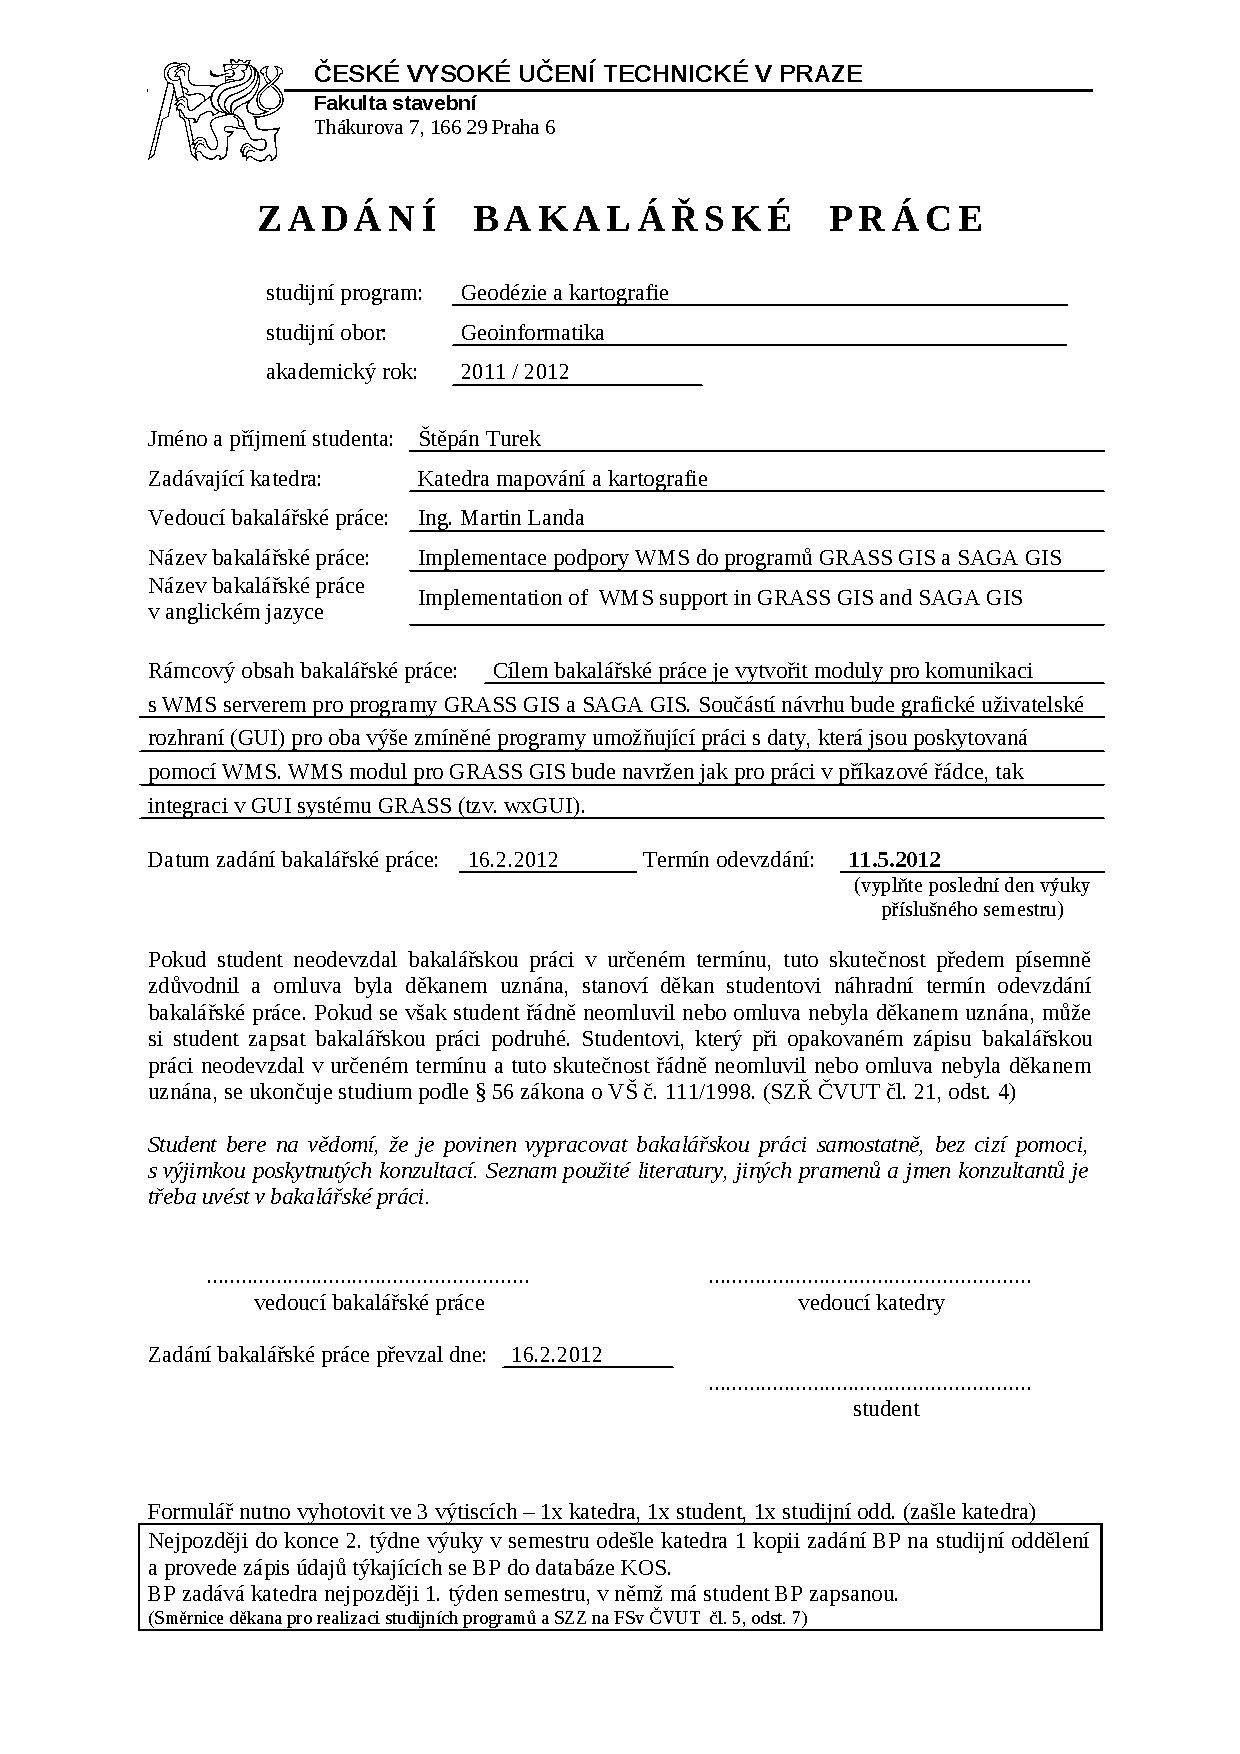
\includepdf[picturecommand={\put(100,200){\vlozZadani}}]{zadani}
 % resi si zalomeni sam





\begin{abstract}

\bigskip

\klicslova{Klíčová slova}{GIS, GRASS, SAGA}

\end{abstract}

\selectlanguage{english}
\begin{abstract}

\bigskip

\klicslova{Keywords}{GIS, GRASS, SAGA}

\end{abstract}
\selectlanguage{czech}


\newpage
\newcommand{\odsaditodzhora}{\hskip1pt\vfill}

\odsaditodzhora
\noindent Prohlášení



\begin{flushleft}
\begin{tabular}{cp{0.3\textwidth}c}
V Praze dne .................
& 
&
..................................
\\
&&
(podpis autora)
\end{tabular}

\end{flushleft}
\newpage

\odsaditodzhora
\noindent Poděkování


\newpage

\newpage
\tableofcontents


\newpage
\pagestyle{fancy}

\necislovana{Úvod}



GRASS GIS (\url{http://grass.osgeo.org}) je geografický informační systém, šířený  pod svobodnou licencí GNU GPL.  
Historie GRASS GIS sahá do roku 1982. V tomto roce americká armáda začala vyvíjet software, který by ji pomohl se správou rozsáhlých oblastí z pohledu ochrany 
životního prostředí, jenž byly kladeny novou legislativou na majitelé pozemků.
 
Významným milníkem pro GRASS je rok 1995, kdy se americká armáda z toho projektu stáhla a kolem GRASS GIS se začala rodit komunita dobrovolníků. 
Dnes je komunita vývojářů rozprostřena po celém světě, z nichž se většina rekrutuje z univerzit a výzkumných ústavů. 

GRASS je jeden z nejrobustnějších svobodných GIS software. Umožnuje pracovat s vektorovými a rastrovými daty.
Jelikož se GRASS se vyvíjí již 25 let, jedním z dědictví takto dlouhého vývoje je, že  jádro je napsáno procedurálně v jazyce C. 
V poslední době je snaha vývojářů učinit GRASS použitelnější pro méně pokročilé uživatele. Z tohoto důvodu bylo vyvinuto nové GUI, které se intenzivně rozvíji. 
Funkcionality GRASS GIS jsou do programu implementovány v podobě modulů. Moduly jsou do programu integrovány pomocí API, které existuje v C a Python verzi.

SAGA GIS\footnote{\url{http://www.saga-gis.org/}} je menší open source projekt, jehož vývoj začal na
 univerzitě v Goettingenu. Nyní je projekt šířen pod  licencí GNU GPL. Vývojařská 
komunita je mezinárodní s těžištěm na domovské universitě. Hlavní síla SAGA GIS spočívá v práci s rastrovými daty. Program je schopen pracovat i s daty vektorovými. 
SAGA GIS je napsán v jazyce  C++.  Koncept programu je rovněž modulární. Moduly jsou do jádra integrovány pomocí API v jazyce C++.

Web Map Service (WMS) je standard\footnote{\url{http://www.opengeospatial.org/standards/wms}}, který definuje rozhraní mezi klientem 
a serverem pro získávání georeferencovaných dat v rastrových formátech \footnote{ vektorová data ve formátu SVG nebo CGM.} (např. JPEG, TIFF, PNG). 
Jde o otevřený standart, který je vyvíjen organizací Open Geospatial Consortium\footnote{\url{http://www.opengeospatial.org/}}.  


\newpage
\section{Stručný úvod do WMS}

Komunikace mezi klientem a serverem probíhá pomocí protokolu HTTP, kdy klient zašle serveru požadavek, 
server požadavek zpracuje a  zašle klientu soubor s odpovědí, což může být rastr v požadovaném formátu nebo soubor s metadaty.

WMS standard je definován v několika verzích.

\begin{table}[h]
\centering
\begin{tabular}{|c|c|c|c|}      \hline
  Číslo verze  & Rok vydání  \\ \hline
  1.0.0        &  2000       \\ \hline
  1.1.0        &  2001       \\ \hline
  1.1.1        &  2002       \\ \hline
  1.3.0        &  2004       \\ \hline
\end{tabular}
\caption{Verze WMS}
\label{tab:verze}
\end{table}

V dnešní době téměř všechny severy podporují verze 1.3.0 a 1.1.1. Protože
změny ve verzi 1.3.0 nejsou uvedeny ve standardu, jsou popsány v příloze [TODO odkaz].


\subsection{Komunikace klient-server}


Požadavak klienta na WMS server může být zaslán pomocí dotazovacích metod GET a POST protokolu HTTP. Pomocí těchto metod je klient schopen
serveru předat parametry, na základě kterých server vytvoří odpověď. WMS standard vyžaduje podporu metody GET, zatímco podpora metody POST je volitelná. 

HTTP GET:

Metoda GET předává parametry jako součást URL. URL adresa  je řetězec znaků, který reprezentuje adresu zdroje informací. Tento řetězec má pevně danou strukturu:
	
\begin{alltt}\footnotesize
	protokol://SERVER: port / cesta k dokumentu ? parametry
\end{alltt}
	
čemuž odpovídá tento příklad WMS dotazu metodou GET:

\begin{alltt}\footnotesize
\url{http://wms.cuzk.cz:80/wms.asp?REQUEST=GetCapabilities&VERSION=1.1.1}
\end{alltt}

\newpage

Protože port číslo 80 je implicitní pro protokol HTTP, není třeba ho zadávat.   
Aby server byl schopen zpracovat část s parametry, jsou určeny znaky (viz. tab \ref{tab:myfirsttable}) se speciálními funkcemi. 

\begin{table}[h]
\centering
\begin{tabular}{|c|l|}      \hline
  Znak      &    Funkce				\\ \hline
   ?        &  Začátek řetězce parametrů.      	\\ \hline
   \&       &  Oddělovač parametrů.   		\\ \hline
   =        &  Oddělovač názvu parametrů a hodnoty.    \\ \hline
   ,        &  Oddělovač jednotlivých položek pokud parametr obsahuje více hodnot\\ \hline
   +        &  Reprezentuje mezeru. 	\\ \hline
\end{tabular}
\caption{Znaky v URL se speciální funkcí}
\label{tab:myfirsttable}
\end{table}

Pokud je potřeba v URL uvést tyto vyhrazené znaky, lze použít URL kódování\footnote{\url{hhttp://www.w3schools.com/tags/ref_urlencode.asp}}.

HTTP POST:

Metoda POST neposílá parametry v URL adrese ale přenáší je v těle POST zprávy.


\subsection{Komunikace server-klient}

Odpovědí servru na WMS dotaz je soubor, který se odesílá protokolem Multipurpose Internet Mail Extensions\footnote{\url{http://mgrand.home.mindspring.com/mime.html}}. Tento protokol umožnuje zasílat soubory pomocí protokolu HTTP.


\subsection{Fungování WMS v praxi}

 
Nejčastěji uživatel získává data z WMS serveru pomocí klienta, který je součástí GIS nebo jiného programu. Každý klient na pozadí vytváří WMS dotazy a jejich 
tvorba je v této kapitole popsána na reálných příkladech. 


\newpage
Jediné, co je potřeba pro zahájení komunikace s WMS serverem, je jeho URL. V tomto případě:
\begin{alltt}\footnotesize
\url{http://geoportal.cuzk.cz/WMS_ZABAGED_PUB/WMService.aspx}
\end{alltt}

Nyní musí klient vytvořit dotaz typu GetCapabilities, aby zjistil informace o datech, která server poskytuje a o parametrech pro ostatní WMS dotazy (GetMap a GetFeatureInfo).
Toto učiní přidáním parametrů k URL adrese WMS serveru:

\newcommand{\CUZKgetCap}{http://geoportal.cuzk.cz/WMS_ZABAGED_PUB/WMService.aspx?SERVICE=WMS&REQUEST=GetCapabilities&VERSION=1.3.0}
\begin{alltt}\footnotesize
\href{\CUZKgetCap}{http://geoportal.cuzk.cz/WMS_ZABAGED_PUB/WMService.aspx?}
\href{\CUZKgetCap}{SERVICE=WMS&REQUEST=GetCapabilities&VERSION=1.3.0}
\end{alltt}

 Dotaz typu GetCapabilities obsahuje parametry, které jsou společne pro všechny typy, protože definují způsob komunikace.
\begin{itemize}
  \item Parametr SERVICE sděluje serveru že se jedná o WMS dotaz. 
  \item Parametr REQUEST popisuje typ dotazu. 
  \item Parametr VERSION popisuje jaká verze WMS standartu bude použita.
\end{itemize}

Aby byl server schopen správně zpracovat WMS dotazy, musí se klient a server dohodnout na verzi WMS, ve které bude probíhat následná komunikace.
Toto je součástí dotazu typu GetCapabilities. Pokud není v dotazu GetCapabilities parametr VERSION, server odpoví ve formátu nejvyšší podporované verze. 
Pokud klient požaduje explicitně určitou verzi, server odpoví v dané verzi, pokud ji podporuje. Jak bylo výše zmíněno, dnes naprostá většina serverů podporuje 
verze 1.1.1 a 1.3.0. Pokud klient podporuje tyto dvě verze, problém s nekompatibilitou v podstatě odpadá.

Na tento dotaz server vrátí soubor ve formátu XML. 

Informace o verzi je uvedena jako atribut úvodního kořenového elementu:
\begin{alltt}\footnotesize
<WMS_Capabilities...    ...version="1.3.0">
\end{alltt}

Kořenový element obsahuje elementy <Service> a <Capability>.

Element  <Service> obsahuje informace o WMS Serveru a poskytovateli dat.
Druhý element <Capability> je mnohem důležitější, protože poskytuje všechny informace, které jsou potřeba pro další komunikaci s WMS serverem.

\begin{alltt}\footnotesize
<Capability>
    <Request>
          ...
       <GetMap>
            <Format>image/png</Format>
            <Format>image/jpeg</Format>
          ...
       </GetMap>	
       <GetFeatureInfo>
            <Format>text/html</Format>
            <Format>text/xml</Format>
              ...
       </GetFeatureInfo>
           ....
\end{alltt}
V této částí jsou uvedeny formáty odpovědí ve tvaru protokolu MIME pro dotaz typu GetMap a GetFeatureInfo. V tomto případě WMS server poskytuje  mapy jako rastry ve formátu PNG, JPEG a další a na 
dotaz typu GetFeatureInfo může vrátit odpověď ve formátu html nebo xml.  

Velmi důležitý je element <Layer>, který obsahuje inforamace o mapové vrstvě. Všechny vrstvy jsou uspořádány do stromové struktury s jedním kořenovým elementem.

\begin{alltt}\footnotesize
<Capability>
    ...
  <Layer>
   <Title>ZABAGED</Title>
     <CRS>EPSG:3035</CRS>
     <CRS>EPSG:3034</CRS>
     <CRS>EPSG:4326</CRS>
      ...
     <BoundingBox CRS="EPSG:3035" minx="4434628.0972282" miny="2778319.58676976"
                                  maxx="4987359.29769667" maxy="3190250.19895492"/>
     <BoundingBox CRS="EPSG:3034" minx="4109720.95957183" miny="2382975.60863023"
                                  maxx="4643932.77142764" maxy="2780500.92255097"/>
      ...
\end{alltt}

Zde jsou uvedeny název kořenové vrstvy <Title> a projekce <CRS> v nichž je dostupná. Název vrstvy se uvádí pomocí elementů <Title> a <Name>. Element
<Title> je název vrstvy ve formátu pro člověka pochopitelném a má pouze informativní charakter, zatímco element <Name> slouží jako unikátní klíč, 
pod kterým je možné danou vrstvu jednoznačně identifikovat v rámci WMS serveru. Jelikož kořenová vrstva nemá element <Name>, není možno poslat požadavek na data této vrstvy. Vrstvy, které neposkytují 
žádná data, se uvádí z důvodu dědičnosti. 

Jelikož projekce je atribut, který je v rámci stromu vrstev děděn a jde o kořenový element, jsou všechny vrstvy dostupné projekcích uvedených v kořenové vrstvě ZABAGED.
Jakákoliv vrstva v tomto stromu může mít definovány další projekce, které budou děděny všemi jejími následovníky ve stromu. 

Element <BoundingBox> reprezentuje obdélník definovaný minimálními a maximálními souřadnicemi v systému projekce uvedené v atributu CRS, který vymezuje rozsah poskytovaných dat. 
Tento element se také ve stromu dědí, pokud je však v potomcích vrstvy nově defininován pro stejnou projekci, nahrazuje děděný element.

 Právě dědičnost je důvodem, proč jsou vrstvy uspořádány do stromové struktury. Díky této struktuře není potřeba v tomto případě u každé vrstvy
uvádět všech 16 souřadnicových systému a obdélníků, čímž dochází k úspoře dat, která jsou přenášena mezi serverem a klientem a také k větší přehlednosti a stručnosti XML souboru.

\newpage

\begin{alltt}\footnotesize
<Capability>
  <Layer>
    <Title>Kořenová vrstva bez dat, chybí name></Title>
    <Layer>
      <Layer>
        <Title>Vrstva č. 1</Title>
        <Name>vrstva1</Name>
      </Layer>
    <Layer>
    <Layer>
      <Layer>
        <Title>Vrstva č. 2</Title>
        <Name>vrstva2</Name>
        <Layer>
          <Title>Vrstva č. 3</Title>
          <Name>vrstva3</Name>
        </Layer>
        <Layer>
          <Title>Vrstva č. 3</Title>
          <Name>vrstva4</Name>
        </Layer>
      </Layer>
    </Layer>
</Capability>
\end{alltt}



Tato delší ukázka ilustruje uspořádání vrstev ve stromové struktuře. Kořenová vrstva se větví v první úrovní  na vrstvy vrstva1, 
vrstva2. Vrstvy vrstva1, vrstva3 a vrstva4 jsou tzv. listy stromu. Takto se nazývají elememnty ve stromové struktuře, které nemají 
žádné potomky. 



\begin{alltt}\footnotesize

<Layer queryable="0" opaque="false" noSubsets="0">
    <Name>GR_CR4</Name>
    <Title>MČR 1 : 1 000 000</Title>
    <Style>
        <Name>Default</Name>
        <Title>Default</Title>
          ...
    </Style>
</Layer>
\end{alltt}


Každá vrsta reprezentuje určitá data, která však mohou být zobrazená rozličnými způsoby. Zbůsob zobrazení definuje tag style. V tomto případě  je pro vrstvu MČR 1 : 1 000 000 
dostupný pouze jeden styl. Vztah elementů <Name> a <Title> pro <Style> je stejný jako v elementu <Layer>.

Díky dotazu GetCapabilities máme všechny potřebné informace k získání požadovaných dat z WMS serveru. 
Toto provedeme pomocí dotazu typu GetMap, v tomto tvaru:



\newcommand{\CUZKgetMap}{http://geoportal.cuzk.cz/WMS_ZABAGED_PUB/WMService.aspx?SERVICE=WMS&REQUEST=GetMap&VERSION=1.3.0&LAYERS=GR_CR4&STYLES=Default&FORMAT=image/png&CRS=EPSG:4326&BBOX=48.093144621684,11.6163532829661,51.4980192528993,19.0628256634265&WIDTH=800&HEIGHT=600}
\begin{alltt}\footnotesize
\href{\CUZKgetMap}{http://geoportal.cuzk.cz/WMS\_ZABAGED\_PUB/WMService.aspx?}
\href{\CUZKgetMap}{SERVICE=WMS\&REQUEST=GetMap\&VERSION=1.3.0\&}
\href{\CUZKgetMap}{LAYERS=GR\_CR4\&STYLES=Default\&FORMAT=image/png\&CRS=EPSG:4326\&}
\href{\CUZKgetMap}{BBOX=48.093144621684,11.6163532829661,51.4980192528993,19.0628256634265\&}
\href{\CUZKgetMap}{WIDTH=800\&HEIGHT=600}
\end{alltt}


\begin{itemize}
  \item Parametr FORMAT definuje formát v němž bude vygenerována odpověď s mapou. 
  \item Parametr LAYERS obsahuje požadované vrstvy. Pořadí v jakém budou vrstvy ve výsledné mapě zobrazeny se uvádí v pořadí v jakém jsou uvedeny. Názvy jednotlivých vrstev 
        jsou odděleny čárkou. Vrstva která je ve uvedena vlevo od dalších vrstev je zobrazena nad těmito vrstvami.
  \item Parametru STYLES obsahuje styly vybraných vrstev. Styly se uvádí ve stejném pořadí jako vrstvy.    
  \item Paramentr CRS definuje projekci výsledné mapy. 
  \item Parametr BBOX určuje v jednotkách požadované projekce obdélník, ve kterém požadujeme data. Hodnoty mohou být i vně obdélníku definovaném v GetCapabilites,
	kde pouze informuje o rozsahu poskytovaných dat.  
  \item Parametry WIDTH a HEIGHT definuje počet pixelů výsledného obrázku. 
\end{itemize}

Všechny tyto parametry byly zvoleny na základě informací, které jsme získali pomocí dotazu GetCapabilities. 

Na základě tohoto dotazu obdržíme jako odpověď rastr ve formátu PNG s přehledovou mapou České republiky:

 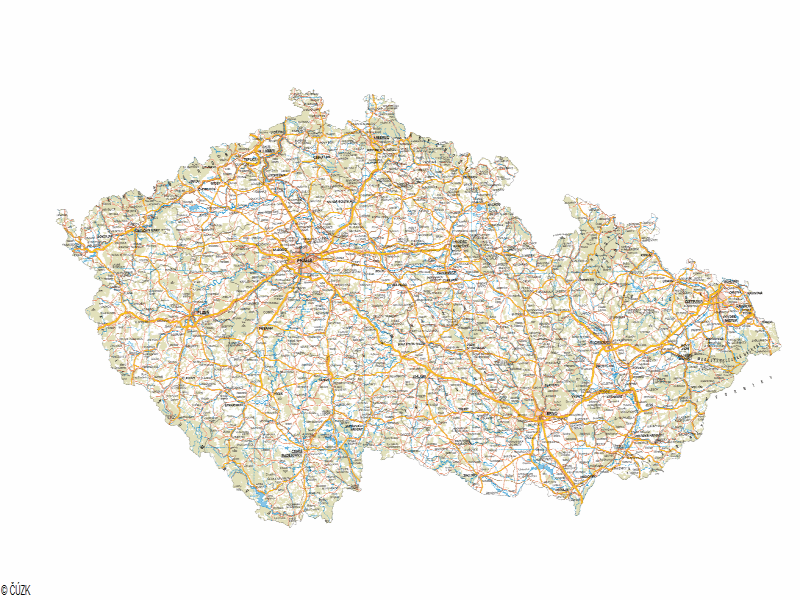
\includegraphics[scale=0.5]{figures/GetMapResponse}


Poslední typ dotazu je volitelný a nazývá se GetFeatureInfo. Ten dotaz, narozdíl od předchozích, nemusí server podporovat.
Dotaz slouží k získán informací o prvcích ve vrstvě.Pokud je v elementu <Layer> uveden argument  queryable 
s hodnotou 1 je možné na tuto vrstvu aplikovat dotaz GetFeatureInfo.  

Jako příklad pro tento typ dotazu je použit WMS server Středočeského kraje. Jedna z WMS služeb, které tento server poskytuje, jsou zóny integrvaného dopravního systému dostupné
na :\url{http://mapy.kr-stredocesky.cz/ids_zony_wms}. 
Nejprve dotazem GetaCapabilities se zjistí informace o WMS serveru a jím poskytovaných datech:

\newcommand{\StredoceskygetCap}{http://mapy.kr-stredocesky.cz/ids_zony_wms?SERVICE=WMS&REQUEST=GetCapabilities}
\begin{alltt}\footnotesize
\href{\StredoceskygetCap}{http://mapy.kr-stredocesky.cz/ids\_zony\_wms?}
\href{\StredoceskygetCap}{SERVICE=WMS\&REQUEST=GetCapabilities\&VERSION=1.3.0}
\end{alltt}

Z odpovědi je patrné, že server obsahuje pouze jednu vrstvu Zony SID, se kterou lze dále pracovat, protože její rodičovská vrstva nemá atribut <Name> nutný pro dotazy GetMap a GetFeatureInfo.
Vrstva je dostupná v jediném souřadnicovém systému. Za povšimnutí stojí opakované uvedení souřadnicové systému a stejného obdélníku BoundingBox v němž jsou poskytována data 
jak v kmenové vrstvě, tak v jejím potomku Zony SID. Jelikož se tyto elementy vrstvy dědí, stačilo by je uvést pouze v kořenové vrstvě.

Na základě informací z dotazu GetCapabilities byl vytvořen dotaz GetMap: 

\url{http://mapy.kr-stredocesky.cz/ids_zony_wms?SERVICE=WMS&REQUEST=GetMap&VERSION=1.3.0&FORMAT=image/png&LAYERS=sid_zony&CRS=EPSG:2065&BBOX=-834258.9702,-1129697.611,-651189.0329,-968639.3882&WIDTH=1000&HEIGHT=1000}
%% \begin{alltt}\footnotesize
%% \href{\StredoceskygetMap}{http://mapy.kr-stredocesky.cz/ids\_zony\_wms?}
%% \href{\StredoceskygetMap}{SERVICE=WMS\&REQUEST=GetMap\&VERSION=1.3.0\&}
%% \href{\StredoceskygetMap}{&LAYERS=sid_zony\&FORMAT=image/png&CRS=EPSG:2065\&}
%% \href{\StredoceskygetMap}{BBOX=48.093144621684,11.6163532829661,51.4980192528993,19.0628256634265\&}
%% \href{\StredoceskygetMap}{WIDTH=1000\&HEIGHT=1000}
%% \end{alltt}

A výsledný dotaz GetFeatureInfo vypadá takto:
\newcommand{\StredoceskyGetFeatureInfo}{http://mapy.kr-stredocesky.cz/ids_zony_wms?REQUEST=GetFeatureInfo&VERSION=1.3.0&FORMAT=image/png&LAYERS=sid_zony&CRS=EPSG:2065&BBOX=-834258.9702,-1129697.611,-651189.0329,-968639.3882&WIDTH=1000&HEIGHT=1000&INFO_FORMAT=text/html&I=695&J=720&QUERY_LAYERS=sid_zony}
\begin{alltt}\footnotesize
\href{\StredoceskyGetFeatureInfo}{http://mapy.kr-stredocesky.cz/ids\_zony\_wms?}
\href{\StredoceskyGetFeatureInfo}{REQUEST=GetFeatureInfo\&VERSION=1.3.0\&}
\href{\StredoceskyGetFeatureInfo}{FORMAT=image/png\&LAYERS=sid\_zony\&CRS=EPSG:2065\&}
\href{\StredoceskyGetFeatureInfo}{BBOX=-834258.9702,-1129697.611,-651189.0329,-968639.3882\&WIDTH=1000\&HEIGHT=1000\&}
\href{\StredoceskyGetFeatureInfo}{INFO\_FORMAT=text/html\&I=695\&J=720\&QUERY\_LAYERS=sid\_zony}
\end{alltt}


Jak lze vidět, tento dotaz zarnuje dotaz GetMap a další parametry:
\begin{itemize}
  \item Parametr REQUEST uvádí typ dotazu GetFeatureInfo 
  \item INFO\_FORMAT tento parametr uvádí formát odpovědi na tento dotaz. WMS standatd neuvádí implicitní formát, který musí server podporovat. V tomto případě se jedná o html soubor. 
  \item Parametry I a J lokalizují prvek, na který se v dotazu GetFeatureInfo ptáme. Tyto souřadnice reprezentují souřadnicový systém obrázku s jednotkami v pixelech a začátkem v levém horním rohu. Souřadnice os I, J narůstají  
        směrem vpravo resp. dolů. Interval souřadnic je dán parametry WIDTH a HEIGHT, kdy I, J mají rozsah od 0 do WIDTH - 1 resp. od 0 do HEIGHT - 1.  
  \item QUERY\_LAYERS je výčet vrstev, kterých se týká dotaz GetFeatureInfo. 
\end{itemize}

  
\begin{figure}[h!]
 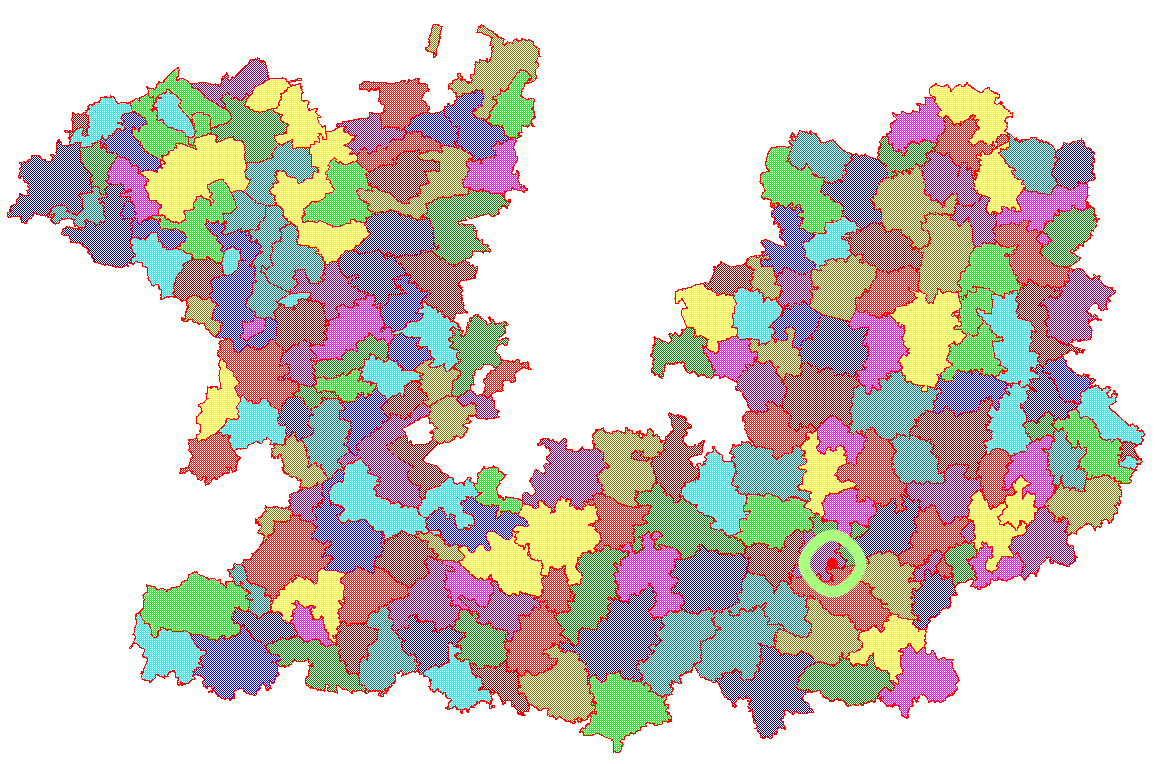
\includegraphics[scale=0.3]{figures/getfeatureinfo}
  \caption{Výsledek GetMap dotazu s bodem o souřadnicích I, J  695 a 720:}
\end{figure}

A jako odpověd obdržíme html dokunent, který se v prohlížeči zobrazí takto:

 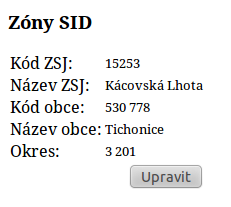
\includegraphics[scale=0.7]{figures/getfeatureinforeply}


Pokud je serveru položen dotaz ve špatném tvaru, vrátí vyjímku implicitně ve formátu XML souboru, v němž je blíže specifikována chyba ve WMS dotazu. 


\newpage

\section{WMS modul pro GRASS}

Jelikož původně GRASS neměl žádné GUI, jeho moduly jsou přispůsobeny pro práci v příkazové řádce. Každý modul si lze představit jako funkci, která má definované vstupní argumenty a určený výstup. Nevýhodou tohoto 
přístupu je že modul není schopen s uživatelem komunikovat za běhu modulu, uživatel může jeho chování ovlivnit jen pomocí argumentů, které jsou zadány před spuštěním. Proto modul pro WMS v GRASS GIS vyhovuje pro implementaci
WMS dotazu typu GetMap. Pomocí modulu nelze zobrazit nabídku parametrů pro dotaz GetMap, která se vygeneruje na základě informací z dotazu GetCapabilities. Toto je potřeba řešit implementací v GUI programů GRASS.



\subsection{Analýza původního stavu}

 V GRASS GIS již existuje modul r.in.wms, který umožňuje získání dat z WMS serveru. Tento modul byl původně napsán jako shell skript. V GRASS 7 byly všechny shell skript moduly přepsány do jazyka Python.      

\end{document}




